% Figure caption + label for the headline §4 Hopf phase diagram.
% Generated by: python -m reflexive_options.experiments.hopf_phase_scan_4d
% Source data:  runs/hopf_phase_scan_4d/<latest>/phase_4d.npz
% Image files:  paper/figures/hopf_phase_diagram.{pdf,png}
%
% Drop into the paper as:
%   \begin{figure}[t]
%       \centering
%       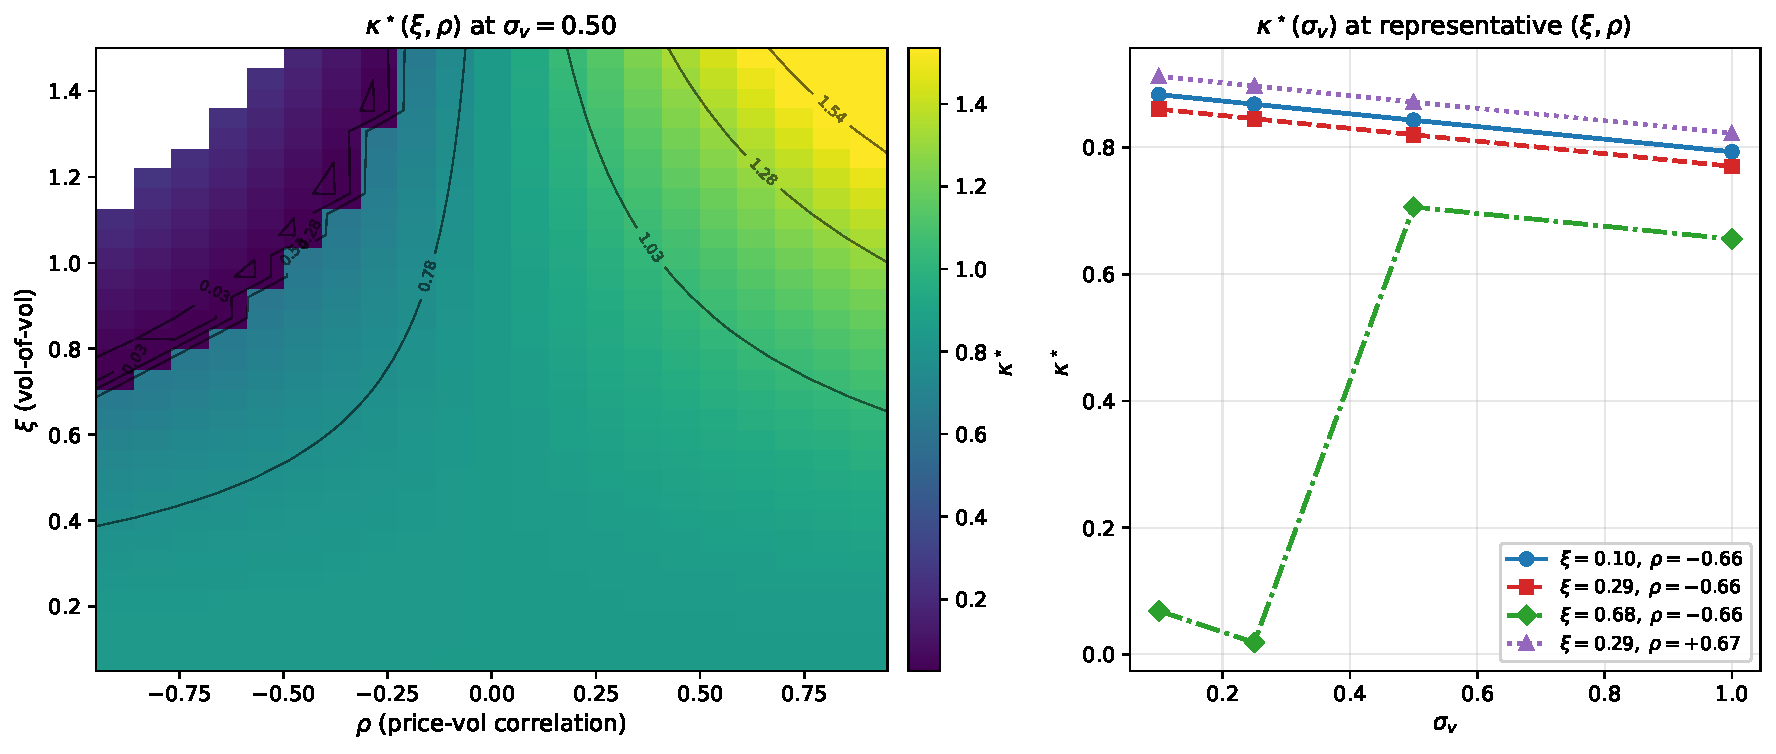
\includegraphics[width=\textwidth]{figures/hopf_phase_diagram.pdf}
%       % Figure caption + label for the headline §4 Hopf phase diagram.
% Generated by: python -m reflexive_options.experiments.hopf_phase_scan_4d
% Source data:  runs/hopf_phase_scan_4d/<latest>/phase_4d.npz
% Image files:  paper/figures/hopf_phase_diagram.{pdf,png}
%
% Drop into the paper as:
%   \begin{figure}[t]
%       \centering
%       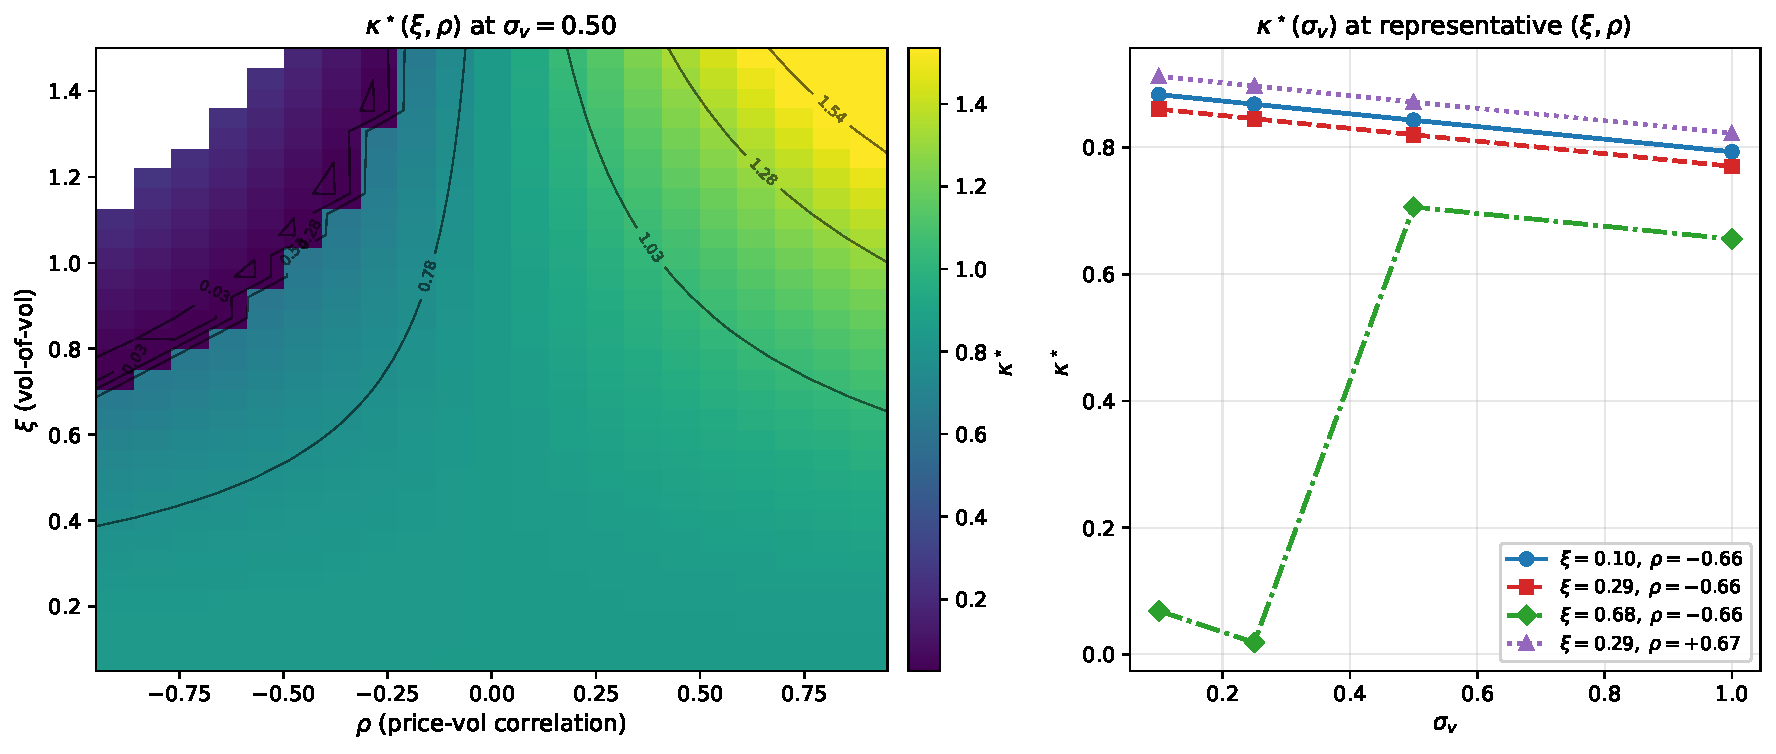
\includegraphics[width=\textwidth]{figures/hopf_phase_diagram.pdf}
%       % Figure caption + label for the headline §4 Hopf phase diagram.
% Generated by: python -m reflexive_options.experiments.hopf_phase_scan_4d
% Source data:  runs/hopf_phase_scan_4d/<latest>/phase_4d.npz
% Image files:  paper/figures/hopf_phase_diagram.{pdf,png}
%
% Drop into the paper as:
%   \begin{figure}[t]
%       \centering
%       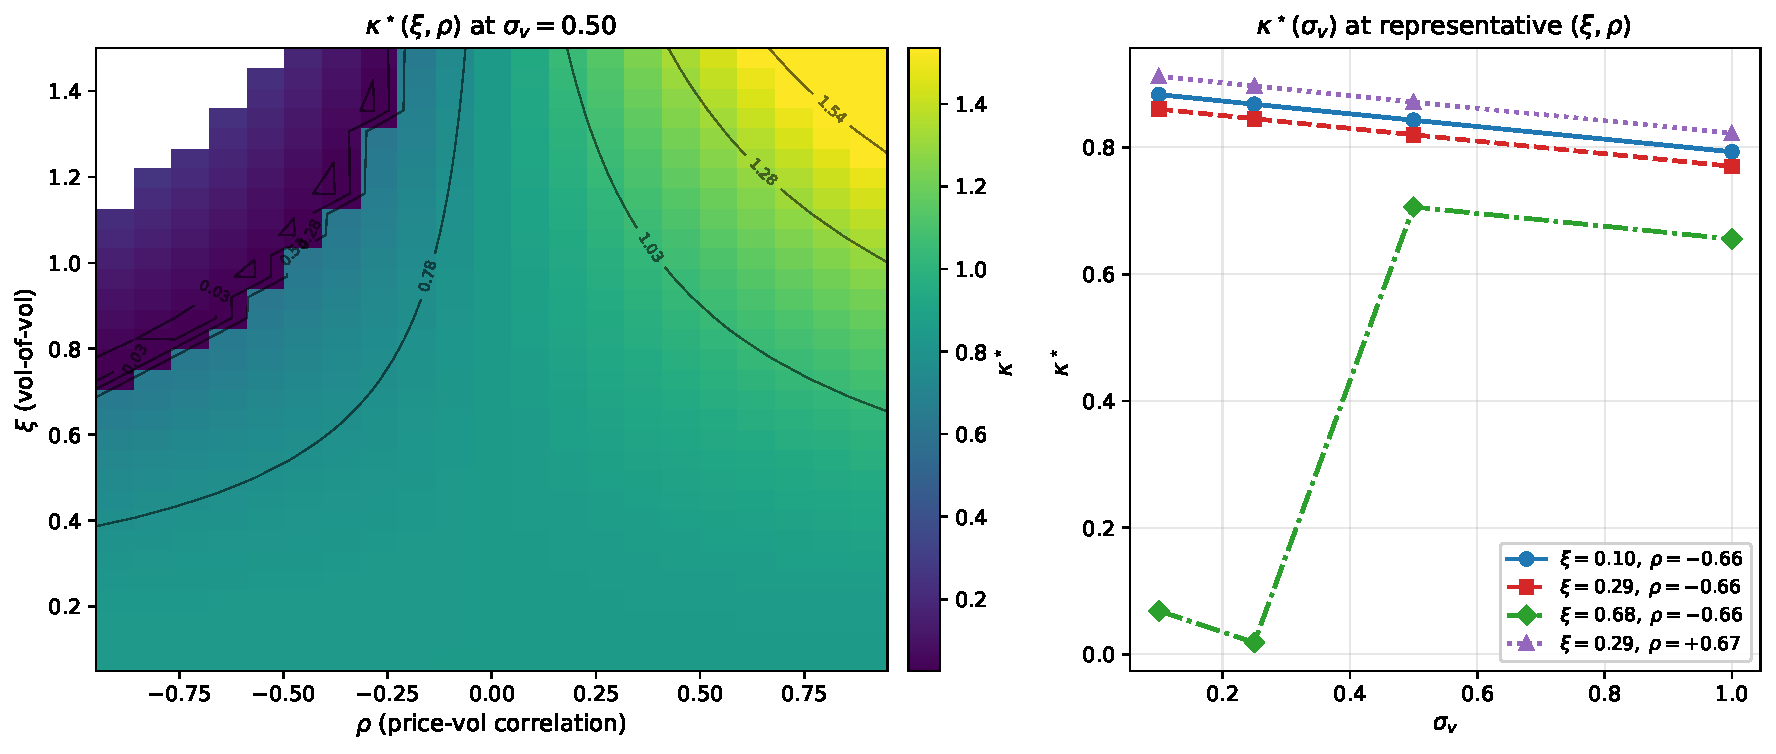
\includegraphics[width=\textwidth]{figures/hopf_phase_diagram.pdf}
%       % Figure caption + label for the headline §4 Hopf phase diagram.
% Generated by: python -m reflexive_options.experiments.hopf_phase_scan_4d
% Source data:  runs/hopf_phase_scan_4d/<latest>/phase_4d.npz
% Image files:  paper/figures/hopf_phase_diagram.{pdf,png}
%
% Drop into the paper as:
%   \begin{figure}[t]
%       \centering
%       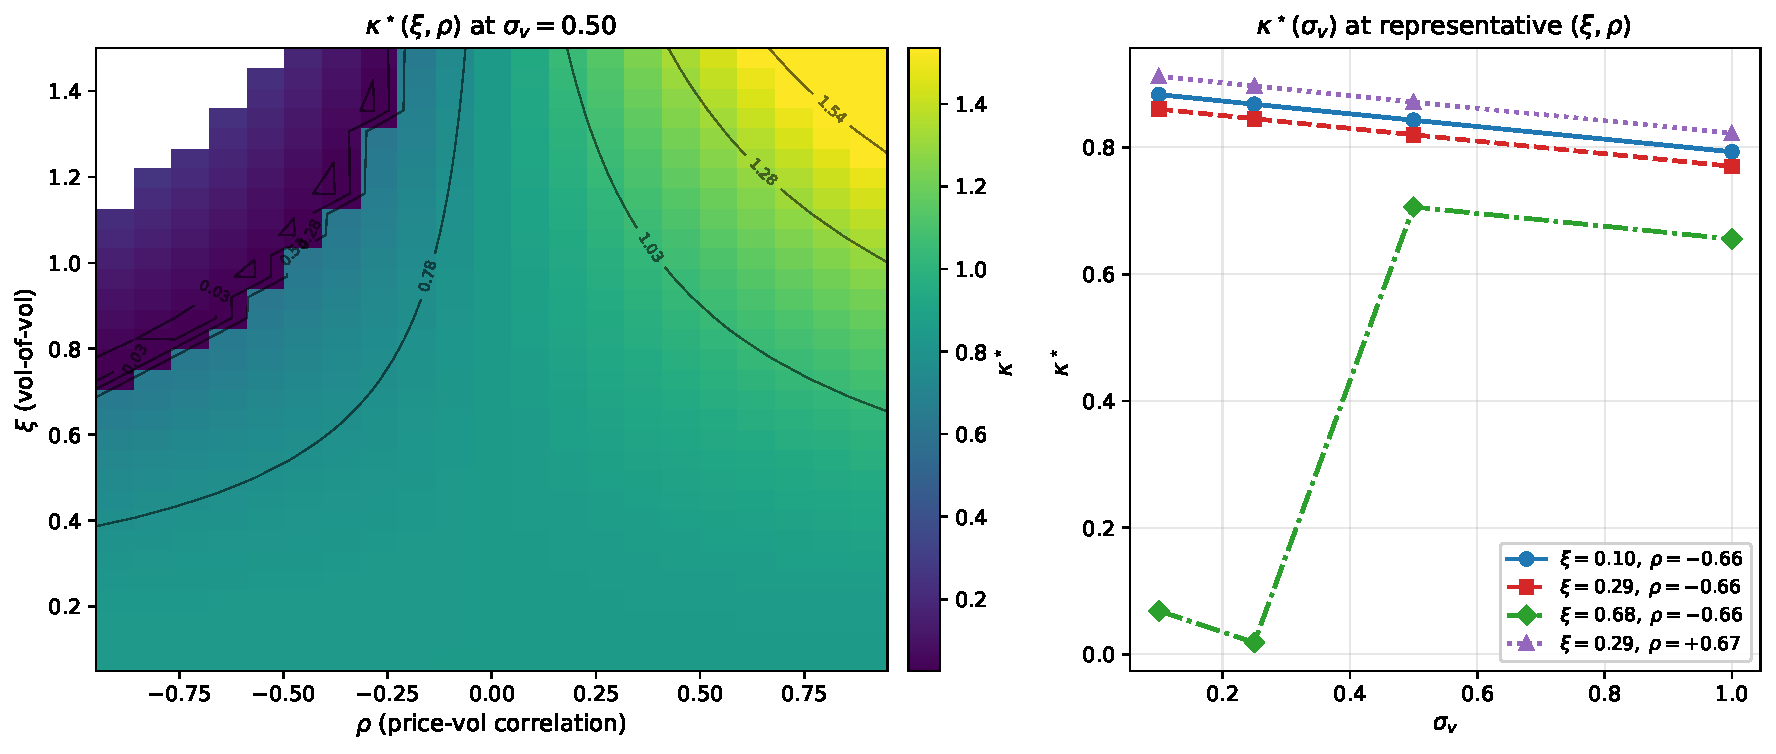
\includegraphics[width=\textwidth]{figures/hopf_phase_diagram.pdf}
%       \input{figures/hopf_phase_diagram.tex}
%   \end{figure}

\caption[Hopf bifurcation threshold over the $(\xi, \rho, \sigma_v)$ slice
of the reflexive parameter space.]{%
    \textbf{Hopf bifurcation threshold $\kappa^\star$ across the
    $(\xi, \rho, \sigma_v)$ slice of the reflexive parameter space.}
    \emph{Left (Panel A):} heatmap of $\kappa^\star(\xi, \rho)$ at the
    median variance-of-variance slice $\sigma_v = 0.50$, computed at the
    canonical Hopf-exhibiting regime of \S\ref{sec:hopf-numerical}
    ($G_x{=}0.5$, $G_v{=}-0.5$, $G_z{=}-0.5$, $\alpha{=}0.5$, $\beta{=}1$,
    $\gamma{=}0.5$, $\kappa_v{=}2$). White cells are configurations with
    no Hopf in the scan range $\kappa \in [0, 2]$ — concentrated in the
    upper-left wedge of high vol-of-vol $\xi$ and strong negative $\rho$,
    where the Engel--Lamb--Rasmussen shear correction destabilises the
    eigenvalue envelope. Contour lines are isoquants of $\kappa^\star$ at
    increments of $(\kappa^\star_{\max} - \kappa^\star_{\min})/6$.
    \emph{Right (Panel B):} four line cuts of $\kappa^\star(\sigma_v)$ at
    representative $(\xi, \rho)$ probes: $(0.10, -0.70)$,
    $(0.30, -0.70)$, $(0.70, -0.70)$, and $(0.30, +0.70)$. The first
    three trace how moving radially outward in vol-of-vol at fixed
    SPX-like $\rho < 0$ pulls the Hopf threshold down; the last
    confirms that flipping $\rho$ to $+0.70$ at moderate $\xi$ keeps
    $\kappa^\star$ in the $0.85$--$0.95$ band. The full scan
    ($31 \times 21 \times 4 = 2{,}604$ cells, each a $401$-point
    $\kappa$-sweep) runs in $\sim$16~s on a single M-series core; reproduce
    via \texttt{python -m reflexive\_options.experiments.hopf\_phase\_scan\_4d}.
}
\label{fig:hopf-phase-diagram}

%   \end{figure}

\caption[Hopf bifurcation threshold over the $(\xi, \rho, \sigma_v)$ slice
of the reflexive parameter space.]{%
    \textbf{Hopf bifurcation threshold $\kappa^\star$ across the
    $(\xi, \rho, \sigma_v)$ slice of the reflexive parameter space.}
    \emph{Left (Panel A):} heatmap of $\kappa^\star(\xi, \rho)$ at the
    median variance-of-variance slice $\sigma_v = 0.50$, computed at the
    canonical Hopf-exhibiting regime of \S\ref{sec:hopf-numerical}
    ($G_x{=}0.5$, $G_v{=}-0.5$, $G_z{=}-0.5$, $\alpha{=}0.5$, $\beta{=}1$,
    $\gamma{=}0.5$, $\kappa_v{=}2$). White cells are configurations with
    no Hopf in the scan range $\kappa \in [0, 2]$ — concentrated in the
    upper-left wedge of high vol-of-vol $\xi$ and strong negative $\rho$,
    where the Engel--Lamb--Rasmussen shear correction destabilises the
    eigenvalue envelope. Contour lines are isoquants of $\kappa^\star$ at
    increments of $(\kappa^\star_{\max} - \kappa^\star_{\min})/6$.
    \emph{Right (Panel B):} four line cuts of $\kappa^\star(\sigma_v)$ at
    representative $(\xi, \rho)$ probes: $(0.10, -0.70)$,
    $(0.30, -0.70)$, $(0.70, -0.70)$, and $(0.30, +0.70)$. The first
    three trace how moving radially outward in vol-of-vol at fixed
    SPX-like $\rho < 0$ pulls the Hopf threshold down; the last
    confirms that flipping $\rho$ to $+0.70$ at moderate $\xi$ keeps
    $\kappa^\star$ in the $0.85$--$0.95$ band. The full scan
    ($31 \times 21 \times 4 = 2{,}604$ cells, each a $401$-point
    $\kappa$-sweep) runs in $\sim$16~s on a single M-series core; reproduce
    via \texttt{python -m reflexive\_options.experiments.hopf\_phase\_scan\_4d}.
}
\label{fig:hopf-phase-diagram}

%   \end{figure}

\caption[Hopf bifurcation threshold over the $(\xi, \rho, \sigma_v)$ slice
of the reflexive parameter space.]{%
    \textbf{Hopf bifurcation threshold $\kappa^\star$ across the
    $(\xi, \rho, \sigma_v)$ slice of the reflexive parameter space.}
    \emph{Left (Panel A):} heatmap of $\kappa^\star(\xi, \rho)$ at the
    median variance-of-variance slice $\sigma_v = 0.50$, computed at the
    canonical Hopf-exhibiting regime of \S\ref{sec:hopf-numerical}
    ($G_x{=}0.5$, $G_v{=}-0.5$, $G_z{=}-0.5$, $\alpha{=}0.5$, $\beta{=}1$,
    $\gamma{=}0.5$, $\kappa_v{=}2$). White cells are configurations with
    no Hopf in the scan range $\kappa \in [0, 2]$ — concentrated in the
    upper-left wedge of high vol-of-vol $\xi$ and strong negative $\rho$,
    where the Engel--Lamb--Rasmussen shear correction destabilises the
    eigenvalue envelope. Contour lines are isoquants of $\kappa^\star$ at
    increments of $(\kappa^\star_{\max} - \kappa^\star_{\min})/6$.
    \emph{Right (Panel B):} four line cuts of $\kappa^\star(\sigma_v)$ at
    representative $(\xi, \rho)$ probes: $(0.10, -0.70)$,
    $(0.30, -0.70)$, $(0.70, -0.70)$, and $(0.30, +0.70)$. The first
    three trace how moving radially outward in vol-of-vol at fixed
    SPX-like $\rho < 0$ pulls the Hopf threshold down; the last
    confirms that flipping $\rho$ to $+0.70$ at moderate $\xi$ keeps
    $\kappa^\star$ in the $0.85$--$0.95$ band. The full scan
    ($31 \times 21 \times 4 = 2{,}604$ cells, each a $401$-point
    $\kappa$-sweep) runs in $\sim$16~s on a single M-series core; reproduce
    via \texttt{python -m reflexive\_options.experiments.hopf\_phase\_scan\_4d}.
}
\label{fig:hopf-phase-diagram}

%   \end{figure}

\caption[Hopf bifurcation threshold over the $(\xi, \rho, \sigma_v)$ slice
of the reflexive parameter space.]{%
    \textbf{Hopf bifurcation threshold $\kappa^\star$ across the
    $(\xi, \rho, \sigma_v)$ slice of the reflexive parameter space.}
    \emph{Left (Panel A):} heatmap of $\kappa^\star(\xi, \rho)$ at the
    median variance-of-variance slice $\sigma_v = 0.50$, computed at the
    canonical Hopf-exhibiting regime of \S\ref{sec:hopf-numerical}
    ($G_x{=}0.5$, $G_v{=}-0.5$, $G_z{=}-0.5$, $\alpha{=}0.5$, $\beta{=}1$,
    $\gamma{=}0.5$, $\kappa_v{=}2$). White cells are configurations with
    no Hopf in the scan range $\kappa \in [0, 2]$ — concentrated in the
    upper-left wedge of high vol-of-vol $\xi$ and strong negative $\rho$,
    where the Engel--Lamb--Rasmussen shear correction destabilises the
    eigenvalue envelope. Contour lines are isoquants of $\kappa^\star$ at
    increments of $(\kappa^\star_{\max} - \kappa^\star_{\min})/6$.
    \emph{Right (Panel B):} four line cuts of $\kappa^\star(\sigma_v)$ at
    representative $(\xi, \rho)$ probes: $(0.10, -0.70)$,
    $(0.30, -0.70)$, $(0.70, -0.70)$, and $(0.30, +0.70)$. The first
    three trace how moving radially outward in vol-of-vol at fixed
    SPX-like $\rho < 0$ pulls the Hopf threshold down; the last
    confirms that flipping $\rho$ to $+0.70$ at moderate $\xi$ keeps
    $\kappa^\star$ in the $0.85$--$0.95$ band. The full scan
    ($31 \times 21 \times 4 = 2{,}604$ cells, each a $401$-point
    $\kappa$-sweep) runs in $\sim$16~s on a single M-series core; reproduce
    via \texttt{python -m reflexive\_options.experiments.hopf\_phase\_scan\_4d}.
}
\label{fig:hopf-phase-diagram}
